\documentclass[tikz,border=2pt]{standalone}
\usepackage{amsmath,amssymb}
\usepackage{tikz}
\usetikzlibrary{positioning}

\begin{document}
% Euler's criterion: a connected network has an Euler tour iff every vertex has even degree.
% Left: all degrees even (tour exists). Right: two odd vertices (no tour; an open Euler
% trail between them exists instead).
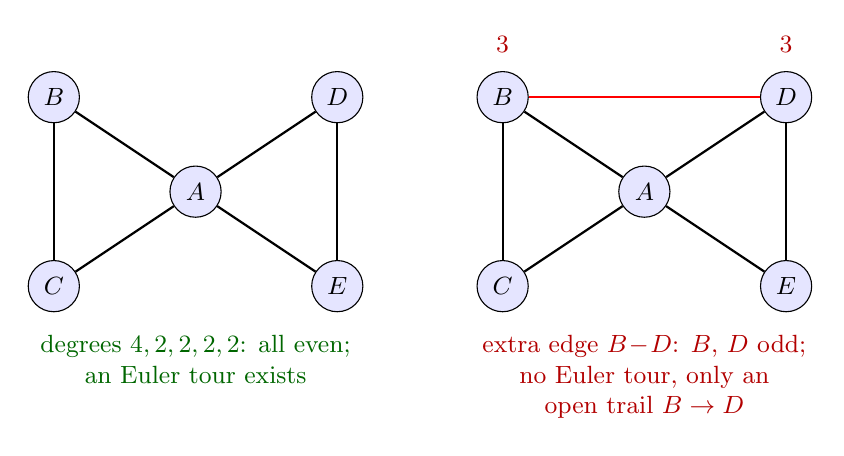
\begin{tikzpicture}[every node/.style={font=\small}, v/.style={draw, circle, fill=blue!10, minimum size=6.5mm, inner sep=0pt}]
	\begin{scope}
		\node[v] (A) at (0,0) {$A$}; \node[v] (B) at (-1.8,1.2) {$B$}; \node[v] (C) at (-1.8,-1.2) {$C$}; \node[v] (D) at (1.8,1.2) {$D$}; \node[v] (E) at (1.8,-1.2) {$E$};
		\foreach \a/\b in {A/B, B/C, C/A, A/D, D/E, E/A} {\draw[thick] (\a) -- (\b);}
		\node[green!40!black, anchor=north, align=center] at (0,-1.7) {degrees $4,2,2,2,2$: all even;\\ an Euler tour exists};
	\end{scope}
	\begin{scope}[xshift=5.7cm]
		\node[v] (A) at (0,0) {$A$}; \node[v] (B) at (-1.8,1.2) {$B$}; \node[v] (C) at (-1.8,-1.2) {$C$}; \node[v] (D) at (1.8,1.2) {$D$}; \node[v] (E) at (1.8,-1.2) {$E$};
		\foreach \a/\b in {A/B, B/C, C/A, A/D, D/E, E/A} {\draw[thick] (\a) -- (\b);}
		\draw[red, thick] (B) -- (D);
		\node[red!70!black, above=3pt of B] {$3$};
		\node[red!70!black, above=3pt of D] {$3$};
		\node[red!70!black, anchor=north, align=center] at (0,-1.7) {extra edge $B\!-\!D$: $B$, $D$ odd;\\ no Euler tour, only an\\ open trail $B\to D$};
	\end{scope}
	\end{tikzpicture}
\end{document}
